\documentclass[tikz,border=2pt]{standalone}
\usepackage{amsmath}
\usepackage{pgfplots}
\pgfplotsset{compat=1.18}
\usepgfplotslibrary{fillbetween}

\begin{document}
% ∫_1^∞ dx/x^p: the tail area is finite for p>1 (the curve drops fast enough) and infinite for p<=1.
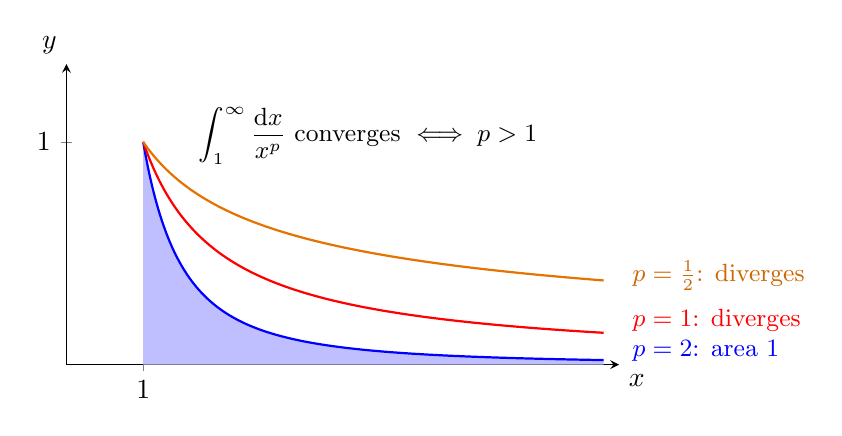
\begin{tikzpicture}
	\begin{axis}[
		axis lines=middle,
		xmin=0, xmax=7.2,
		ymin=0, ymax=1.35,
		xtick={1}, ytick={1},
		xlabel={$x$}, ylabel={$y$},
		xlabel style={below right}, ylabel style={above left},
		samples=200, smooth, clip=false,
		width=8.6cm, height=5.4cm
		]
		\addplot[name path=a, thick, blue, domain=1:7] {1/x^2};
		\addplot[name path=b, thick, red, domain=1:7] {1/x};
		\addplot[name path=c, thick, orange!90!black, domain=1:7] {1/sqrt(x)};
		\addplot[name path=ax, draw=none, domain=1:7] {0};
		\addplot[blue!25] fill between[of=a and ax];
		\node[blue, anchor=west, font=\small] at (axis cs:7.25,0.06) {$p=2$: area $1$};
		\node[red, anchor=west, font=\small] at (axis cs:7.25,0.2) {$p=1$: diverges};
		\node[orange!80!black, anchor=west, font=\small] at (axis cs:7.25,0.4) {$p=\tfrac12$: diverges};
		\node[anchor=north west, font=\small] at (axis cs:1.6,1.2) {$\displaystyle\int_1^{\infty}\frac{\mathrm{d}x}{x^p}$ converges $\iff p>1$};
	\end{axis}
\end{tikzpicture}
\end{document}
